\section{神经网络之反向传播}
\label{sec:chapter8}

\subsection{代价函数}

回顾正则化逻辑回归的代价函数：
\[
J(\theta)=-\frac{1}{m}\left[\sum_{i=1}^my^{(i)}\ln(h_\theta(x^{(i)}))+(1-y^{(i)})\ln(1-h_\theta(x^{(i)}))\right]+\frac{\lambda}{2m}\sum_{j=1}^n\theta_j^2
\]
我们在第四篇中通过极大似然法解释了它的来历，这个代价函数被称作「交叉熵代价函数」，与我们在线性回归中使用的「二次代价函数」形成对比。

在神经网络中，我们沿用交叉熵代价函数。具体地，对于一个 $K$ 分类的神经网络而言，它可以看作是从输入到 $K$ 个二分类输出的过程：$x\mapsto h_\Theta(x)$，我们设其代价函数为每一个二分类的\textbf{交叉熵代价函数之和}：
\[
J(\Theta)=-\frac{1}{m}\left[\sum_{i=1}^m\sum_{k=1}^Ky^{(i)}_k\ln\left(h_\Theta(x^{(i)})_k\right)+(1-y_k^{(i)})\ln\left(1-h_\Theta(x^{(i)})_k\right)\right]+\frac{\lambda}{2m}\sum_{l=1}^{L-1}\sum_{i=1}^{s_l}\sum_{j=1}^{s_{l+1}}\left(\Theta_{ji}^{(l)}\right)^2
\]

其中：$h_\Theta(x^{(i)})\in\mathbb R^K$，表示从第 $i$ 个输入经由神经网络得到的输出结果，$h_\Theta(x^{(i)})_k$ 表示其第 $k$ 维. 

> 注意这里有一个符号混用的地方：上标 $^{(i)}$ 在 $x^{(i)}$ 和 $y^{(i)}$ 中表示第 $i$ 个数据的输入（$\in\mathbb R^{n+1}$）和输出（$\in\mathbb R^{K}$），但是在 $\Theta^{(l)}$ 中表示第 $l$ 层的 $\Theta$（$\in \mathbb R^{s_{l+1}\times (s_l+1)}$）. 

现在我们的目标即是最小化代价函数 $J(\Theta)$，并找到最小时的参数 $\Theta$. 

我们欲使用梯度下降法解决这个问题，所以我们需要计算 $\frac{\partial J}{\partial \Theta_{ji}^{(l)}}$，计算方法就是反向传播算法。

\subsection{反向传播算法}

\paragraph{推导}

为了推导方便，先假设只有一组数据 $(x,y)$，这样可以省去上标和求和的麻烦。我们对第 $l+1$ 层的第 $j$ 个神经元定义一个误差：
\[
\delta_j^{(l+1)}=\frac{\partial J}{\partial z_j^{(l+1)}}
\]
其中 $z_j^{(l+1)}=\sum\limits_{k=0}^{s_{l}}\Theta^{(l)}_{jk}a^{(l)}_{k}$，其实就是把对 $a_j^{(l+1)}$ 的逻辑回归单独拎出来看，取 $\text{sigmoid}$ 前的那个求和值。换句话说，$a^{(l+1)}_j=g\left(z_j^{(l+1)}\right)$. 

于是乎，我们有：
\[
\frac{\partial J}{\partial \Theta^{(l)}_{ji}}=\frac{\partial J}{\partial z_j^{(l+1)}}\cdot\frac{\partial z_j^{(l+1)}}{\partial\Theta_{ji}^{(l)}}=a_i^{(l)}\delta_j^{(l+1)}
\]
写作矩阵形式：
\[
\boxed{\Delta^{(l)}=\delta^{(l+1)}\cdot(a^{(l)})^T}
\]
所以现在问题转化为求解 $\delta^{(l+1)}$. 

采用递推的思想。首先来算输出层，即 $\delta_j^{(L)}$：
\begin{align*}
\delta_j^{(L)}&=\frac{\partial J}{\partial z_j^{(L)}}=\frac{\partial J}{\partial a_j^{(L)}}\cdot\frac{\partial a_j^{(L)}}{\partial z_j^{(L)}}\\
&=\frac{\partial J}{\partial a_j^{(L)}}\cdot g'\left(z_j^{(L)}\right)\\
&=-\left(\frac{y_j}{a_j^{(L)}}-\frac{1-y_j}{1-a_j^{(L)}}\right)\cdot\left(a_j^{(L)}(1-a_j^{(L)})\right)\\
&=a_j^{(L)}-y_j
\end{align*}

所以：
\[
\boxed{\delta^{(L)}=a^{(L)}-y}
\]

\begin{note}
上面推导过程的一些注释：

关于第二行，请注意：$a^{(L)}=g(z^{(L)})$；

关于第三行，请注意 $\text{sigmoid}$ 函数的一个很好的性质：$g'(z)=g(z)(1-g(z))$；

以及，关于偏导项的计算，请注意 $a^{(L)}=h_\Theta(x)$，所以 $J(\Theta)$ 在现在的假设条件下可以写作：
\[
J(\Theta)=-\left[\sum_{k=1}^Ky_k\ln(a^{(L)}_k)+(1-y_k)\ln(1-a_k^{(L)})\right]+\frac{\lambda}{2}\sum_{l=1}^{L-1}\sum_{i=1}^{s_l}\sum_{j=1}^{s_{l+1}}\left(\Theta_{ji}^{(l)}\right)^2
\]
\end{note}


现在计算第 $l$ 层（$2\leqslant l<L$）的 $\delta^{(l)}$：
\begin{align*}
\delta_j^{(l)}&=\frac{\partial J}{\partial z_j^{(l)}}\\
&=\frac{\partial J}{\partial z^{(l+1)}}\cdot\frac{\partial z^{(l+1)}}{\partial a_j^{(l)}}\cdot\frac{\partial a_j^{(l)}}{\partial z_j^{(l)}}\\
&={\delta^{(l+1)}}^T\Theta^{(l)}_{\bullet,j}\cdot g'(z_j^{(l)})\\
&={\delta^{(l+1)}}^T\Theta^{(l)}_{\bullet,j}\cdot \left(a_j^{(l)}*(1-a_j^{(l)})\right)
\end{align*}
所以：
\[
\boxed{\delta^{(l)}=\left({\Theta^{(l)}}^T\delta^{(l+1)}\right)*\left(a^{(l)}*(1-a^{(l)})\right)}
\]
其中 $*$ 表示两个向量对应位置相乘。


\paragraph{步骤总结}

以上是对一组数据的推导，我们得到了三个重要的结果：
\begin{align*}
&\Delta^{(l)}=\delta^{(l+1)}\cdot(a^{(l)})^T&&1\leqslant l<L\\
&\delta^{(L)}=a^{(L)}-y\\
&\delta^{(l)}=\left({\Theta^{(l)}}^T\delta^{(l+1)}\right)*\left(a^{(l)}*(1-a^{(l)})\right)&&2\leqslant l<L
\end{align*}
而 $m$ 组数据只需要在一些地方进行累加即可，具体如下：

设数据集为：$\left\{(x^{(i)},y^{(i)})\mid 1\leqslant i\leqslant m\right\}$，则反向传播算法的步骤为：

\begin{enumerate}
    \item 所有 $\Delta^{(l)}$ 置零；
    \item 遍历数据集，设当前数据为 $(x^{(i)},y^{(i)})$：
        \begin{enumerate}
            \item 以 $x^{(i)}$ 为输入做前向传播，得到输出 $a^{(L)}$；
            \item 置 $\delta^{(L)}=a^{(L)}-y^{(i)}$，进行反向传播：$\delta^{(l)}={\Theta^{(l)}}^T\delta^{(l+1)}*\left[a^{(l)}(1-a^{(l)})\right],\;2\leqslant l<L$；
            \item 更新 $\Delta$ 矩阵：$\Delta^{(l)}:=\Delta^{(l)}+\delta^{(l+1)}\cdot(a^{(l)})^T,\;1\leqslant l<L$；
        \end{enumerate}
    \item 计算 $D$ 矩阵：
       \[
       D_{ij}^{(l)}:=\begin{cases}
       \frac{1}{m}\left(\Delta_{ij}^{(l)}+\lambda\Theta_{ij}^{(l)}\right)&\text{if }j\neq0\\
       \frac{1}{m}\Delta_{ij}^{(l)}&\text{if }j=0
       \end{cases}
       \]
       这就是我们的偏导数矩阵：$\frac{\partial J}{\partial \Theta_{ij}^{(l)}}=D^{(l)}_{ij}$. 
\end{enumerate}

现在，我们可以用 $D_{ij}^{(l)}$ 做梯度下降了。注意一点，我们的参数 $\Theta^{(l)}$ 应该初始化为 $[-\epsilon,\epsilon]$ 中的随机值。


\subsection{梯度检验}

写神经网络反向传播的代码时很容易写 bug，包括一些从结果并不能发现的 bug。梯度检验可以帮助发现这些 bug。

我们可以数值近似 $J(\theta)$ 的各偏导：
\[
\frac{\partial}{\partial \theta_k}J(\theta)\approx\frac{J(\theta_1,\cdots,\theta_k+
\epsilon,\cdots,\theta_n)-J(\theta_1,\cdots,\theta_k-
\epsilon,\cdots,\theta_n)}{2\epsilon}
\]

现在我们可以比较这些偏导估计值与 $D_{ij}^{(l)}$ 对应位置的值，它们应该非常接近。

注意一点：梯度检验耗时巨大，一旦验证了神经网络反向传播的代码正确后，不应进行梯度检验（删掉/注释掉）。


\subsection{代码实现}

这次用的数据集依旧是手写数字识别的数据集，共 $5000$ 组数据，每组数据输入是一个由 $20\times20$ 灰度矩阵压缩而来的 $400$ 维向量，输出是 $0$ 到 $9$ 之间的整数。

\paragraph{第一部分·代价函数与前向传播}

前向传播与上一节的代码没有什么本质的区别，不过这里将其一般化，可适用于 $L$ 层的神经网络且 $m$ 个数据同时计算：

\begin{lstlisting}[language=Python]
def forwardPropagation():
	a = [None] * (L+1)
	a[1] = np.hstack((np.ones((m, 1)), X))
	for l in range(2, L):
		a[l] = sigmoid(np.matmul(a[l-1], Theta[l-1].T))
		a[l] = np.hstack((np.ones((m, 1)), a[l]))
	a[L] = sigmoid(np.matmul(a[L-1], Theta[L-1].T))
	return a
\end{lstlisting}

当然只计算一个数据也是可以的：

\begin{lstlisting}[language=Python]
def forwardPropagation(x):
	"""
	x: (n, 1)
	"""
	a = [None] * (L+1)
	a[1] = np.vstack((np.ones((1, 1)), x))
	for l in range(2, L):
		a[l] = sigmoid(np.matmul(Theta[l-1], a[l-1]))
		a[l] = np.vstack((np.ones((1, 1)), a[l]))
	a[L] = sigmoid(np.matmul(Theta[L-1], a[L-1]))
	return a
\end{lstlisting}

代价函数及其正则化：

\begin{lstlisting}[language=Python]
def J(lamb):
	res = 0
	FP = forwardPropagation()
	res -= np.sum(Y * np.log(FP[L]) + (1-Y) * np.log(1-FP[L]))
	for l in range(1, L):
		res += lamb / 2 * np.sum(np.power(Theta[l][:, 1:], 2))
	res /= m
	return res
\end{lstlisting}

使用 `ex4weights.mat` 中给定的参数 $\Theta$，在无正则化时，准确率为 $97.52\%$，代价为 $0.28762916516131865$；

在正则化时（$\lambda=1$），准确率为 $97.52\%$，代价为 $0.3844877962428937$。


\paragraph{第二部分·反向传播}

反向传播算法：

\begin{lstlisting}[language=Python]
def backPropagation(lamb):
	Delta = [None] * L # (s_{l+1}, s_l+1)
	for l in range(1, L):
		Delta[l] = np.zeros((s[l+1], s[l]+1))
	delta = [None] * (L+1) # (s_l, )
	a = forwardPropagation()
	for i in range(m):
		delta[L] = a[L][i:i+1, :].T - Y[i:i+1, :].T
		for l in range(L-1, 1, -1):
			delta[l] = (np.matmul(Theta[l].T, delta[l+1]) * (a[l][i:i+1, :].T * (1 - a[l][i:i+1, :].T)))[1:, :]
		for l in range(1, L):
			Delta[l] += np.matmul(delta[l+1], a[l][i:i+1, :])
	D = [None] * L # (s_{l+1}, s_l+1)
	for l in range(1, L):
		D[l] = (Delta[l] + lamb * np.hstack((np.zeros((s[l+1], 1)), Theta[l][:, 1:]))) / m
	return D
\end{lstlisting}

梯度下降：

\begin{lstlisting}[language=Python]
def GradientDescent(alpha, iteration):
	for l in range(1, L):
		Theta[l] = np.random.random((s[l+1], s[l]+1))
		Theta[l] = (Theta[l] - 0.5) / 4
	for t in range(iteration):
		D = backPropagation(lamb=1)
		for l in range(1, L):
			Theta[l] -= alpha * D[l]
		Z.append(J(lamb=1))
	return Theta
\end{lstlisting}

梯度检验（把这段代码插入到梯度下降计算出 $D$ 矩阵之后的地方即可）：

\begin{lstlisting}[language=Python]
for l in range(1, L):
    for i in range(s[l+1]):
        for j in range(s[l]+1):
            Theta[l][i, j] -= 0.001
            J1 = J(lamb=1)
            Theta[l][i, j] += 0.002
            J2 = J(lamb=1)
            Theta[l][i, j] -= 0.001
            print(D[l][i, j], (J2 - J1) / 0.002)
\end{lstlisting}

现在我们可以开始训练了！代价随迭代次数增加的变化如下：

\begin{figure}[H]
    \centering
    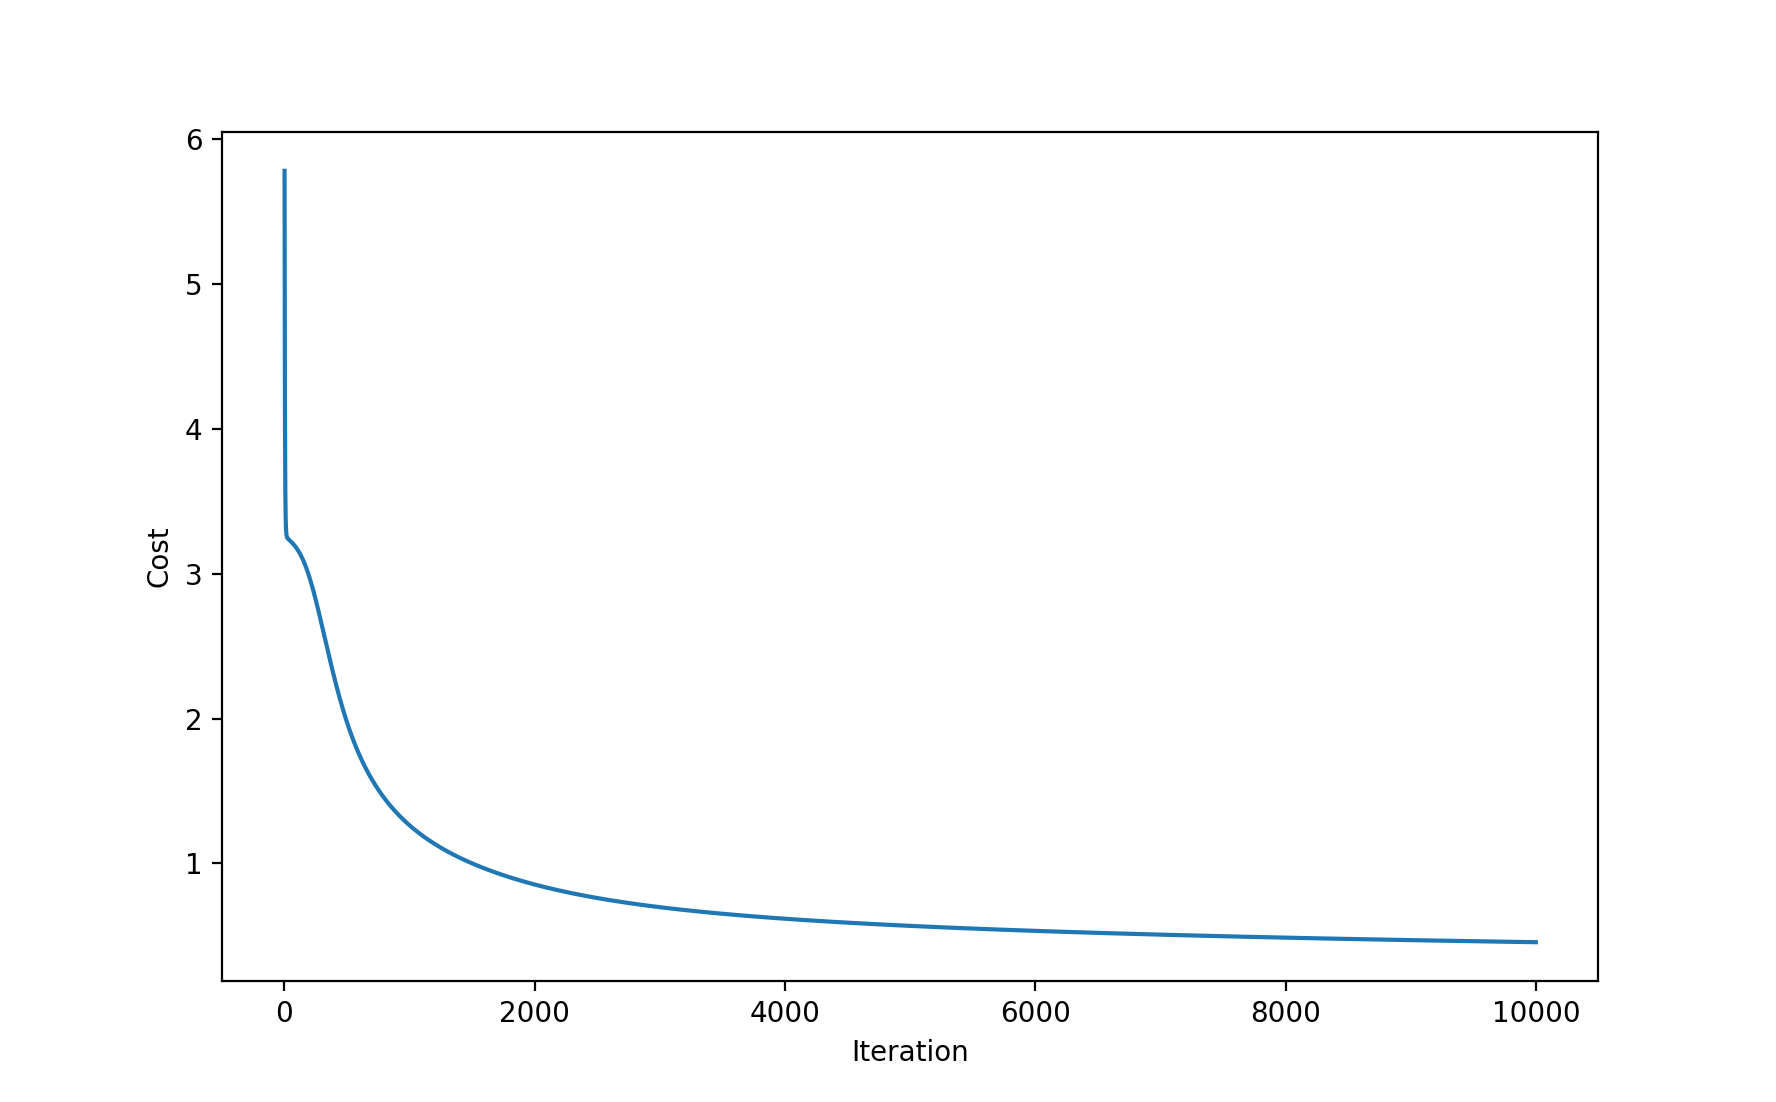
\includegraphics[width=0.5\linewidth]{figs/Chap_8_Figure_1.png}
\end{figure}

准确率如下：

\begin{table}[H]
    \centering
    \small
    \begin{tabularx}{\linewidth}{lYYYYYYYYYYY}
    \toprule
	数字 & 0 & 1 & 2 & 3 & 4 & 5 & 6 & 7 & 8 & 9 & Total \\
    \midrule
	准确率 & 98.6\% & 97.8\% & 93.4\% & 93.4\% & 97.0\% & 93.8\% & 97.8\% & 95.6\% & 95.8\% & 94.0\% & 95.7\% \\
    \bottomrule
    \end{tabularx}
\end{table}

\paragraph{附·使用 \texttt{scipy} 优化}

自己写的梯度下降跑得很慢，使用 \texttt{scipy.optimize.minimize} 来最小化 $J(\Theta)$，method 选用 $\text{CG}$，结果如下：

\begin{lstlisting}
     fun: 0.3139915007113895
     jac: array([-2.06059133e-05, -3.07615047e-11,  7.43614742e-10, ...,
       -2.86333807e-05,  4.03018555e-06,  5.10265929e-05])
 message: 'Optimization terminated successfully.'
    nfev: 1074
     nit: 461
    njev: 1074
  status: 0
 success: True
       x: array([-9.31407860e-01, -1.53807524e-07,  3.71577070e-06, ...,
       -1.27597236e-01, -1.69568829e-01,  3.47560466e-01])
\end{lstlisting}

\begin{figure}[H]
    \centering
    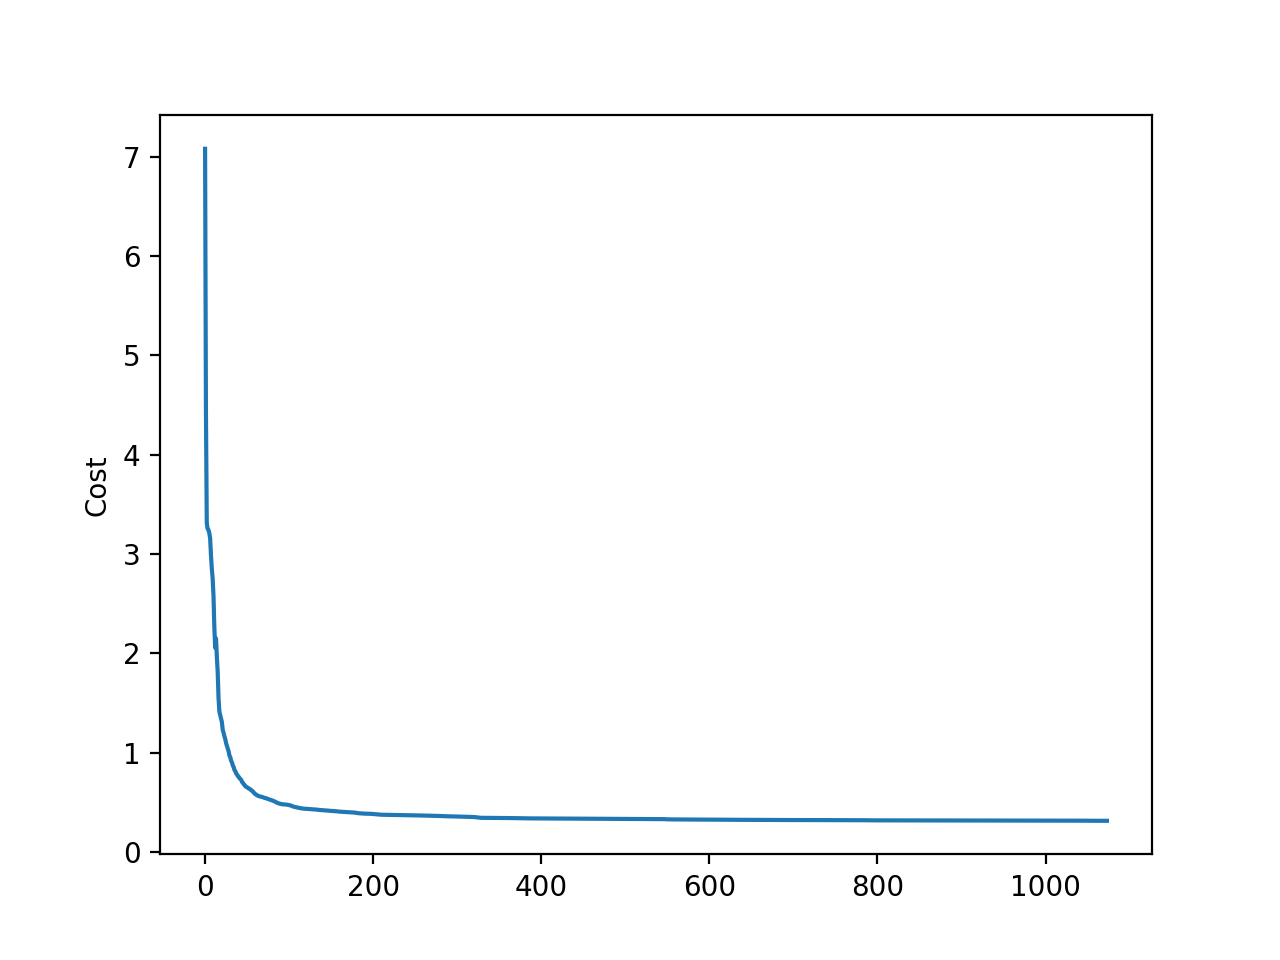
\includegraphics[width=0.5\linewidth]{figs/Chap_8_Figure_CG.png}
\end{figure}

\begin{table}[H]
    \centering
    \small
    \begin{tabularx}{\linewidth}{lYYYYYYYYYYY}
    \toprule
	数字 & 0 & 1 & 2 & 3 & 4 & 5 & 6 & 7 & 8 & 9 & Total \\
    \midrule
	准确率 & 99.8\% & 100.0\% & 99.4\% & 99.4\% & 99.2\% & 99.8\% & 99.6\% & 99.6\% & 100.0\% & 99.0\% & 99.6\% \\
    \bottomrule
    \end{tabularx}
\end{table}

当然，再次强调，由于没有划分训练集、验证集、测试集，这个准确率并不能说明问题。
